\documentclass[12pt]{article}

\usepackage{booktabs}
\usepackage{tabularx}
\usepackage{longtable}
\usepackage{hyperref}
\usepackage{graphicx}
\usepackage[center]{caption}
\usepackage{float}
\captionsetup{justification=centering}

\hypersetup{ bookmarks=true,         % show bookmarks bar?
    colorlinks=true,      % false: boxed links; true: colored links
    linkcolor=red,          % color of internal links (change box color with
    citecolor=green,        % color of links to bibliography
    filecolor=magenta,      % color of file links
    urlcolor=cyan           % color of external links
}

\newcommand{\lips}{\textit{Insert your content here.}}
%% Comments

\usepackage{color}

\newif\ifcomments\commentstrue %displays comments
%\newif\ifcomments\commentsfalse %so that comments do not display

\ifcomments
\newcommand{\authornote}[3]{\textcolor{#1}{[#3 ---#2]}}
\newcommand{\todo}[1]{\textcolor{red}{[TODO: #1]}}
\else
\newcommand{\authornote}[3]{}
\newcommand{\todo}[1]{}
\fi

\newcommand{\wss}[1]{\authornote{blue}{SS}{#1}} 
\newcommand{\plt}[1]{\authornote{magenta}{TPLT}{#1}} %For explanation of the template
\newcommand{\an}[1]{\authornote{cyan}{Author}{#1}}

%% Common Parts

\newcommand{\progname}{Software Engineering} % PUT YOUR PROGRAM NAME HERE
\newcommand{\authname}{Team 21, Alkalytics
\\ Sumanya Gulati - gulats10
\\ Kate Min - mink9
\\ Jennifer Ye - yej52
\\ Jason Tran - tranj78} % AUTHOR NAMES                  

\usepackage{hyperref}
    \hypersetup{colorlinks=true, linkcolor=blue, citecolor=blue, filecolor=blue,
                urlcolor=blue, unicode=false}
    \urlstyle{same}
                                


\title{User Guide for \progname: Alkalytics} 
\author{\authname}
\date{\today}

\begin{document}

\maketitle
\newpage
\tableofcontents
\newpage

\section{Introduction}

This comprehensive document provides complete instructions for installing,
configuring, and using all features of the Alkalytics web application.

\section{System Overview}

This section describes the technical architecture, components, and requirements
for running Alkalytics.

\subsection{Detailed Requirements}

Lists all hardware and software requirements for running the application.

\paragraph{Hardware Requirements}
\begin{table}[H]
    \centering
    \begin{tabularx}{\textwidth}{llX}
        \toprule
        \textbf{Component} & \textbf{Minimum} & \textbf{Recommended} \\
        \midrule
        RAM & 8GB & 16GB \\
        Storage & 5GB & 50GB SSD \\
        Processor & 2 cores & 4 cores \\
        \bottomrule
    \end{tabularx}
\end{table}

\section{Installation Guide}

This section provides complete step-by-step instructions for setting up the
Alkalytics environment.

\subsection{Step-by-Step Installation}
\begin{enumerate}
    \item \textbf{Prerequisite Installation}
    \begin{enumerate}
        \item Install Node.js from \url{https://nodejs.org}
        \item Install MongoDB from \url{https://www.mongodb.com}
        \item Install Python 3.x from \url{https://www.python.org}
    \end{enumerate}
    
    \item \textbf{Repository Setup}
    \begin{verbatim}
    git clone https://github.com/SumanyaG/Alkalytics.git
    \end{verbatim}
    
    \item \textbf{Dependency Installation}
    \begin{verbatim}
    yarn install
    pip install -r requirements.txt
    \end{verbatim}
    
    \item \textbf{Database Configuration}
    \begin{enumerate}
        \item KATE HELP
    \end{enumerate}
    
    \item \textbf{Application Launch}
    \begin{enumerate}
        \item Start backend:
        \begin{verbatim}
            uvicorn api:app --reload --host 127.0.0.1 --port 8000
        \end{verbatim}
        \item Start server:
        \begin{verbatim}
        yarn ts-node src/utils/server.ts
        \end{verbatim}
        \item Start frontend:
        \begin{verbatim}
        yarn start
        \end{verbatim}
    \end{enumerate}
\end{enumerate}

\subsection{Verification}
After installation, verify all components are running:
\begin{enumerate}
    \item Frontend: \texttt{http://localhost:3000}
    \item Server: \texttt{http://localhost:8000/graphql}
    \item Backend: \texttt{http://localhost:8000/docs}
    \item Database: Check MongoDB connection on port 27017
\end{enumerate}

\section{User Management}
\subsection*{Section Overview}
This application has different user roles. Each role has a different set of
permissions and respective capabilities within the application.

\subsection{Admin and Researcher Role}
Administrators have full control over all system functionality including data
management, user configuration, and system settings. Both Admin and Researcher
roles have the same permissions. \newline \newline
These features include:
\begin{itemize}
    \item Editing tables, including modifying cells, adding/removing rows and columns.
    \item Setting data types for columns.
    \item Using the Excel function bar for calculations.
    \item Computing efficiency metrics.
    \item Managing bulk data uploads.
    \item Generating and exporting graphs.
\end{itemize}

\subsection{Researcher Assistant Role}
Researcher assistants can view data, run analyses, and generate reports but have limited
system configuration capabilities. \newline\newline
These features include:
\begin{itemize}
    \item Viewing and searching tables (Experiment, Efficiency, and Raw Data).
    \item Searching within a specific column or the entire table.
    \item Generating graphs but with restricted data modification capabilities.
\end{itemize}

\newpage
\section{Web Application Pages}

\subsection{Login and Sign Up Process}
When users first load onto the page, they will be greated by a log in screen. 
If the user has login credentions, log in as normal 
\begin{figure}[H]
    \centering
    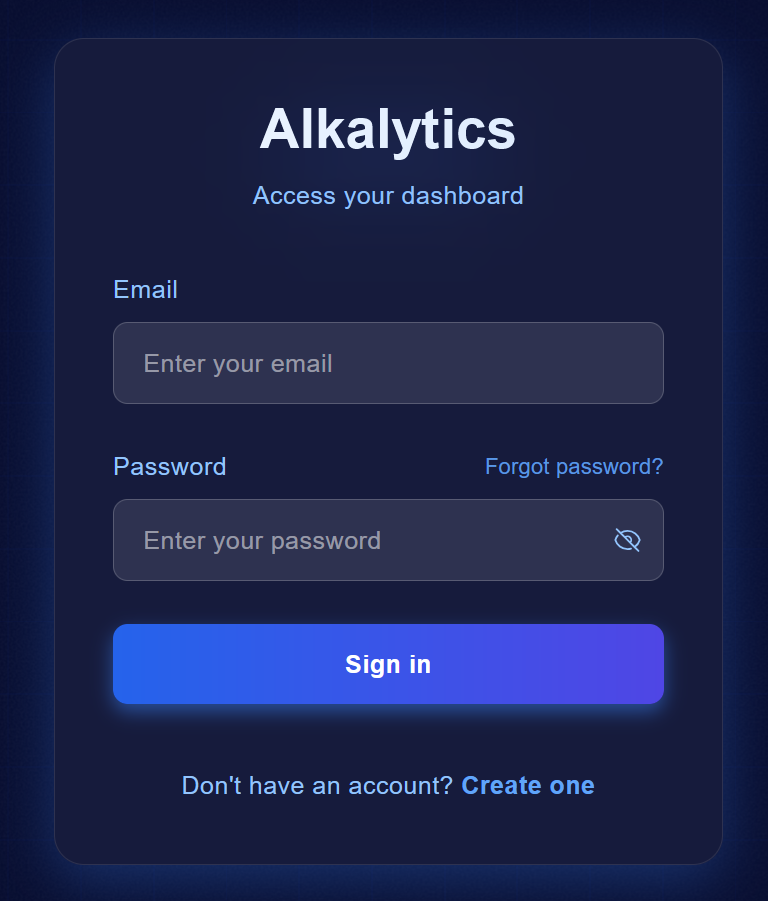
\includegraphics[scale=0.55]{Images/login .png}
    \caption{Login Form}
    \label{fig:example}
\end{figure}

\subsection{Sign Up Process}
If users do not have an account, they will need to create one by clicking the
\textbf{Create one} button at the bottom of the login form. The user must then
enter an email and desired password. There will be three roles to pick from,
Admin, Researcher and Research Assistant. After creating a user account, log in
as normal. 
\begin{figure}[H]
    \centering
    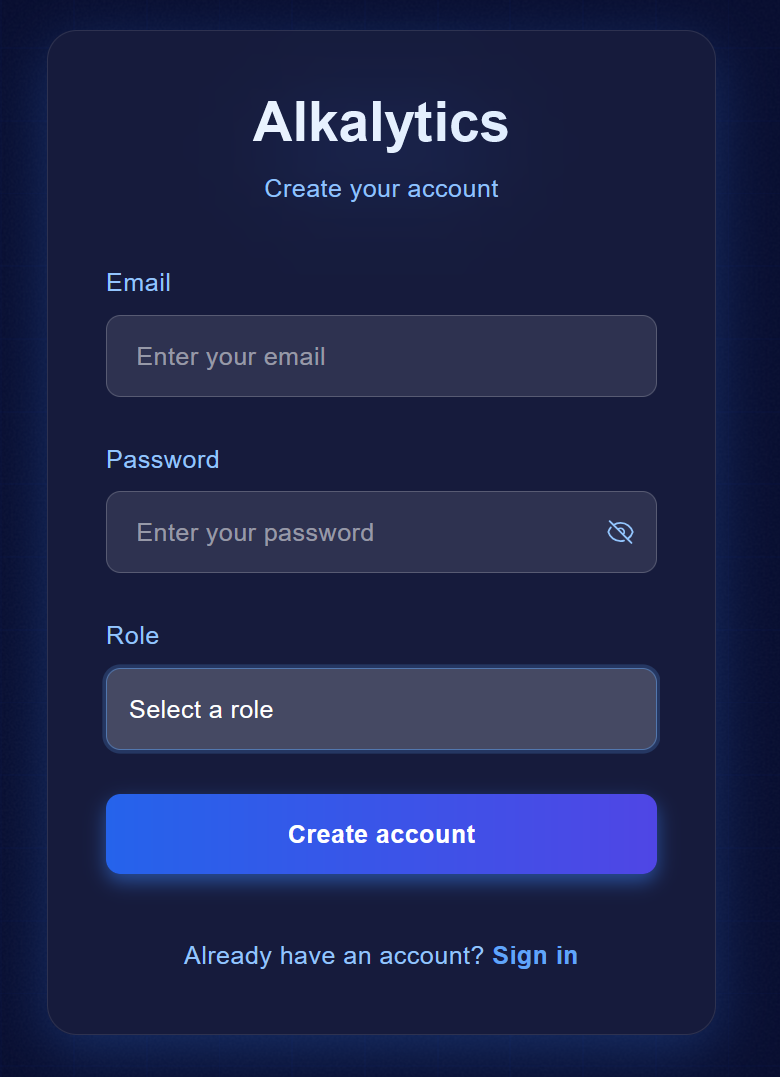
\includegraphics[scale=0.55]{Images/sign up .png}
    \caption{Sign Up Form}
    \label{fig:example}
\end{figure}

\subsection{Upload Process}
\subsubsection*{Description}
The upload functionality allows users to import experimental data in various
formats for analysis.
This section outlines the various pages and functionalities of the web
application, such as uploads, processing, and table management.

\subsection{Dashboard}

The Dashboard provides a quick, interactive, and structured overview of the most
recent key data insights through visualizations and tables. It is designed to
help users analyze trends, monitor performance, and interact with data
efficiently.

\begin{figure}[H]
    \centering
    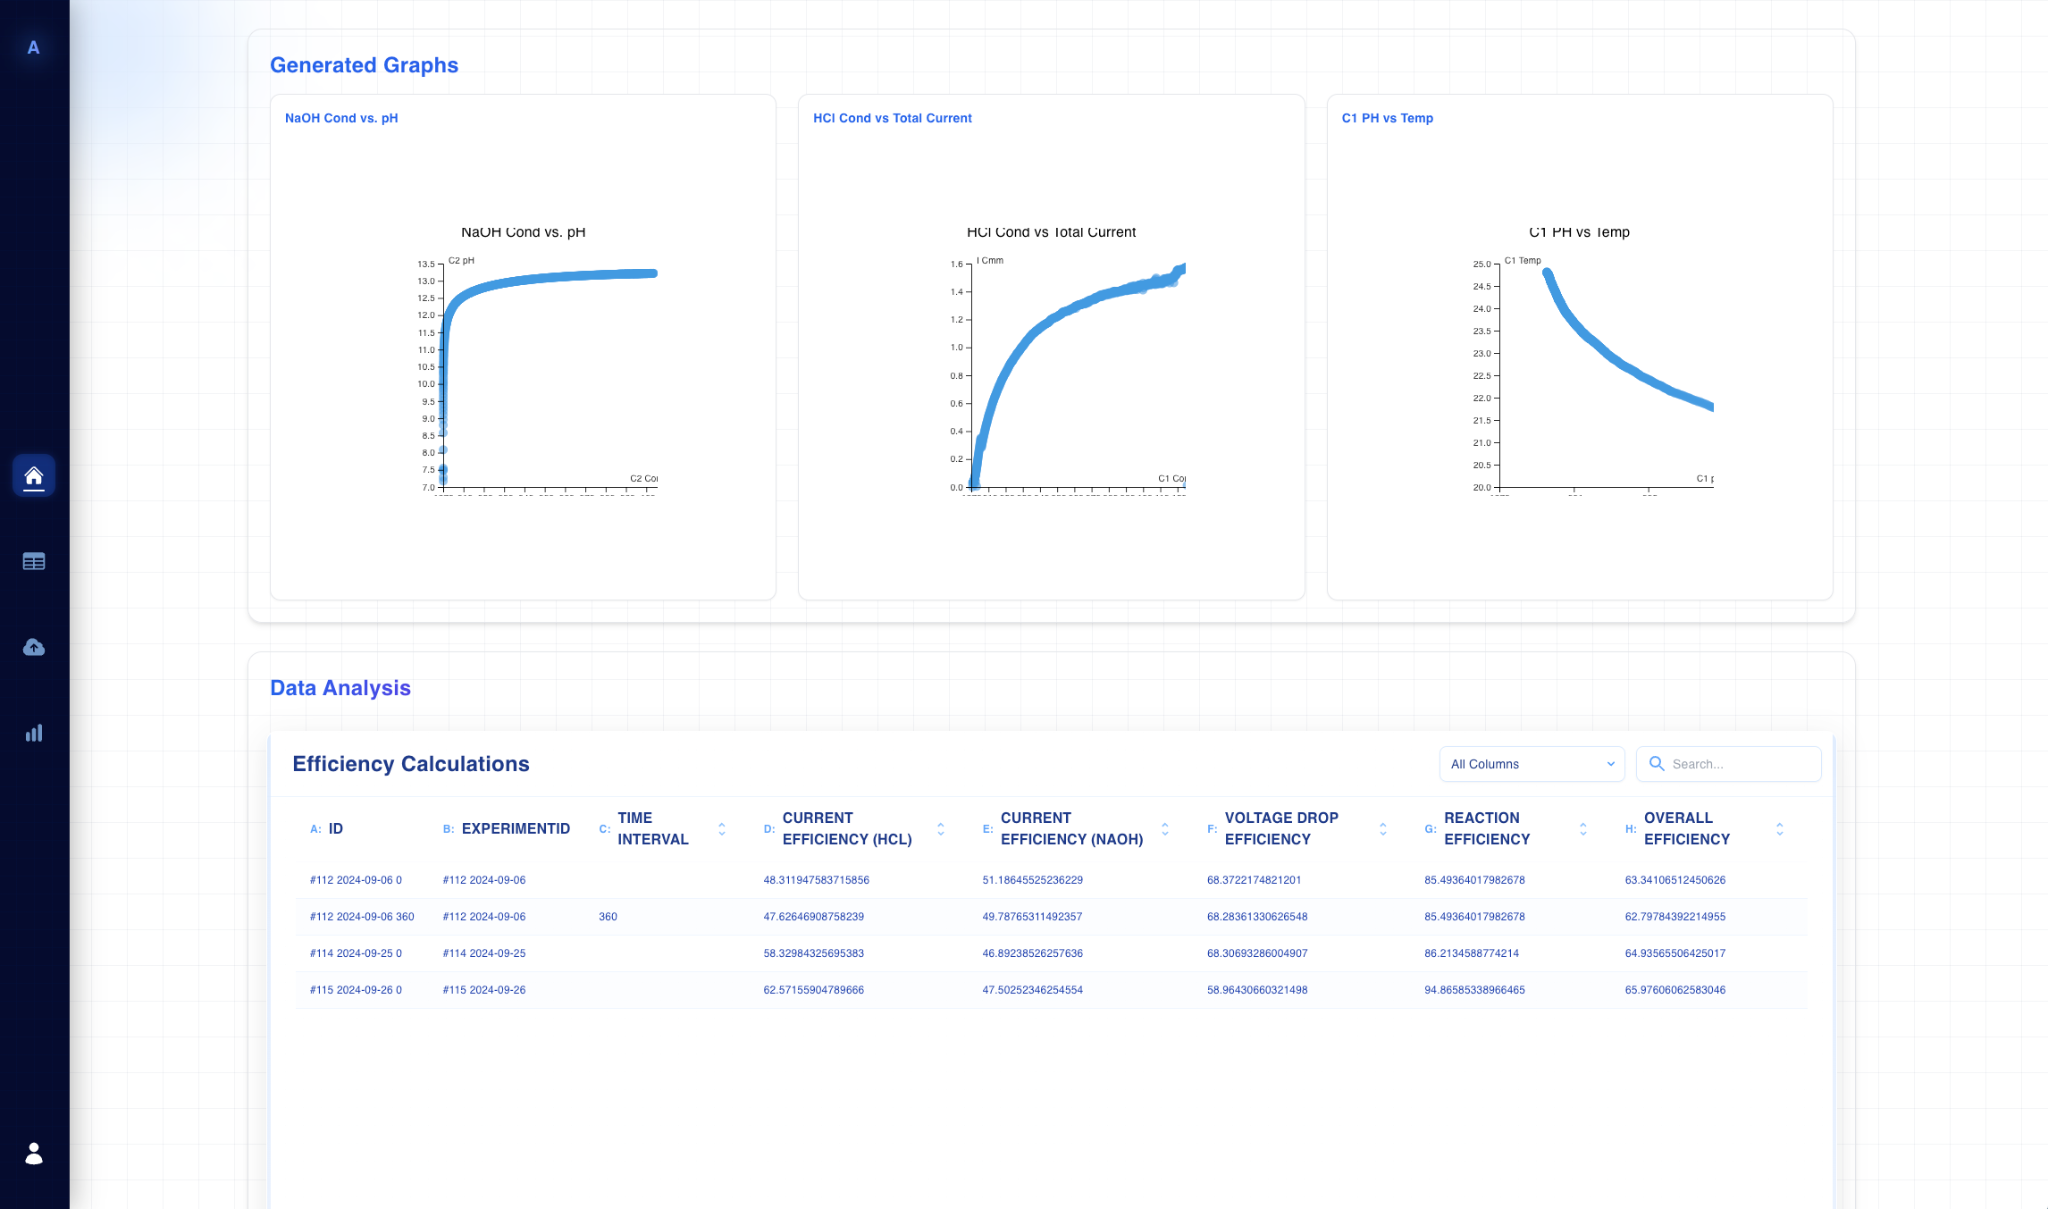
\includegraphics[width=0.8\textwidth]{./Diagrams/Dashboard.png}
    \caption{Dashboard Overview}
\end{figure}


\subsubsection{Key Features}
\begin{itemize}
    \item \textbf{Graphs}: Displays visual representations of data trends and
    relationships.
    \item \textbf{Data Tables}: Organizes numerical and analytical data in a
    structured format, allowing for sorting, filtering, and searching.
    \item \textbf{Navigation Panel}: A sidebar with quick access to different
    sections of the platform, including:
    \begin{itemize}
        \item Dashboard
        \item Data View
        \item Upload
        \item Graphs
        \item Logout
    \end{itemize}
\end{itemize}

\subsection{Upload}

The upload functionality allows users to efficiently import files in various
formats for analysis. This section outlines the steps for uploading files, the
types of files supported, and best practices to ensure a smooth upload
experience.

\begin{figure}[H]
    \centering
    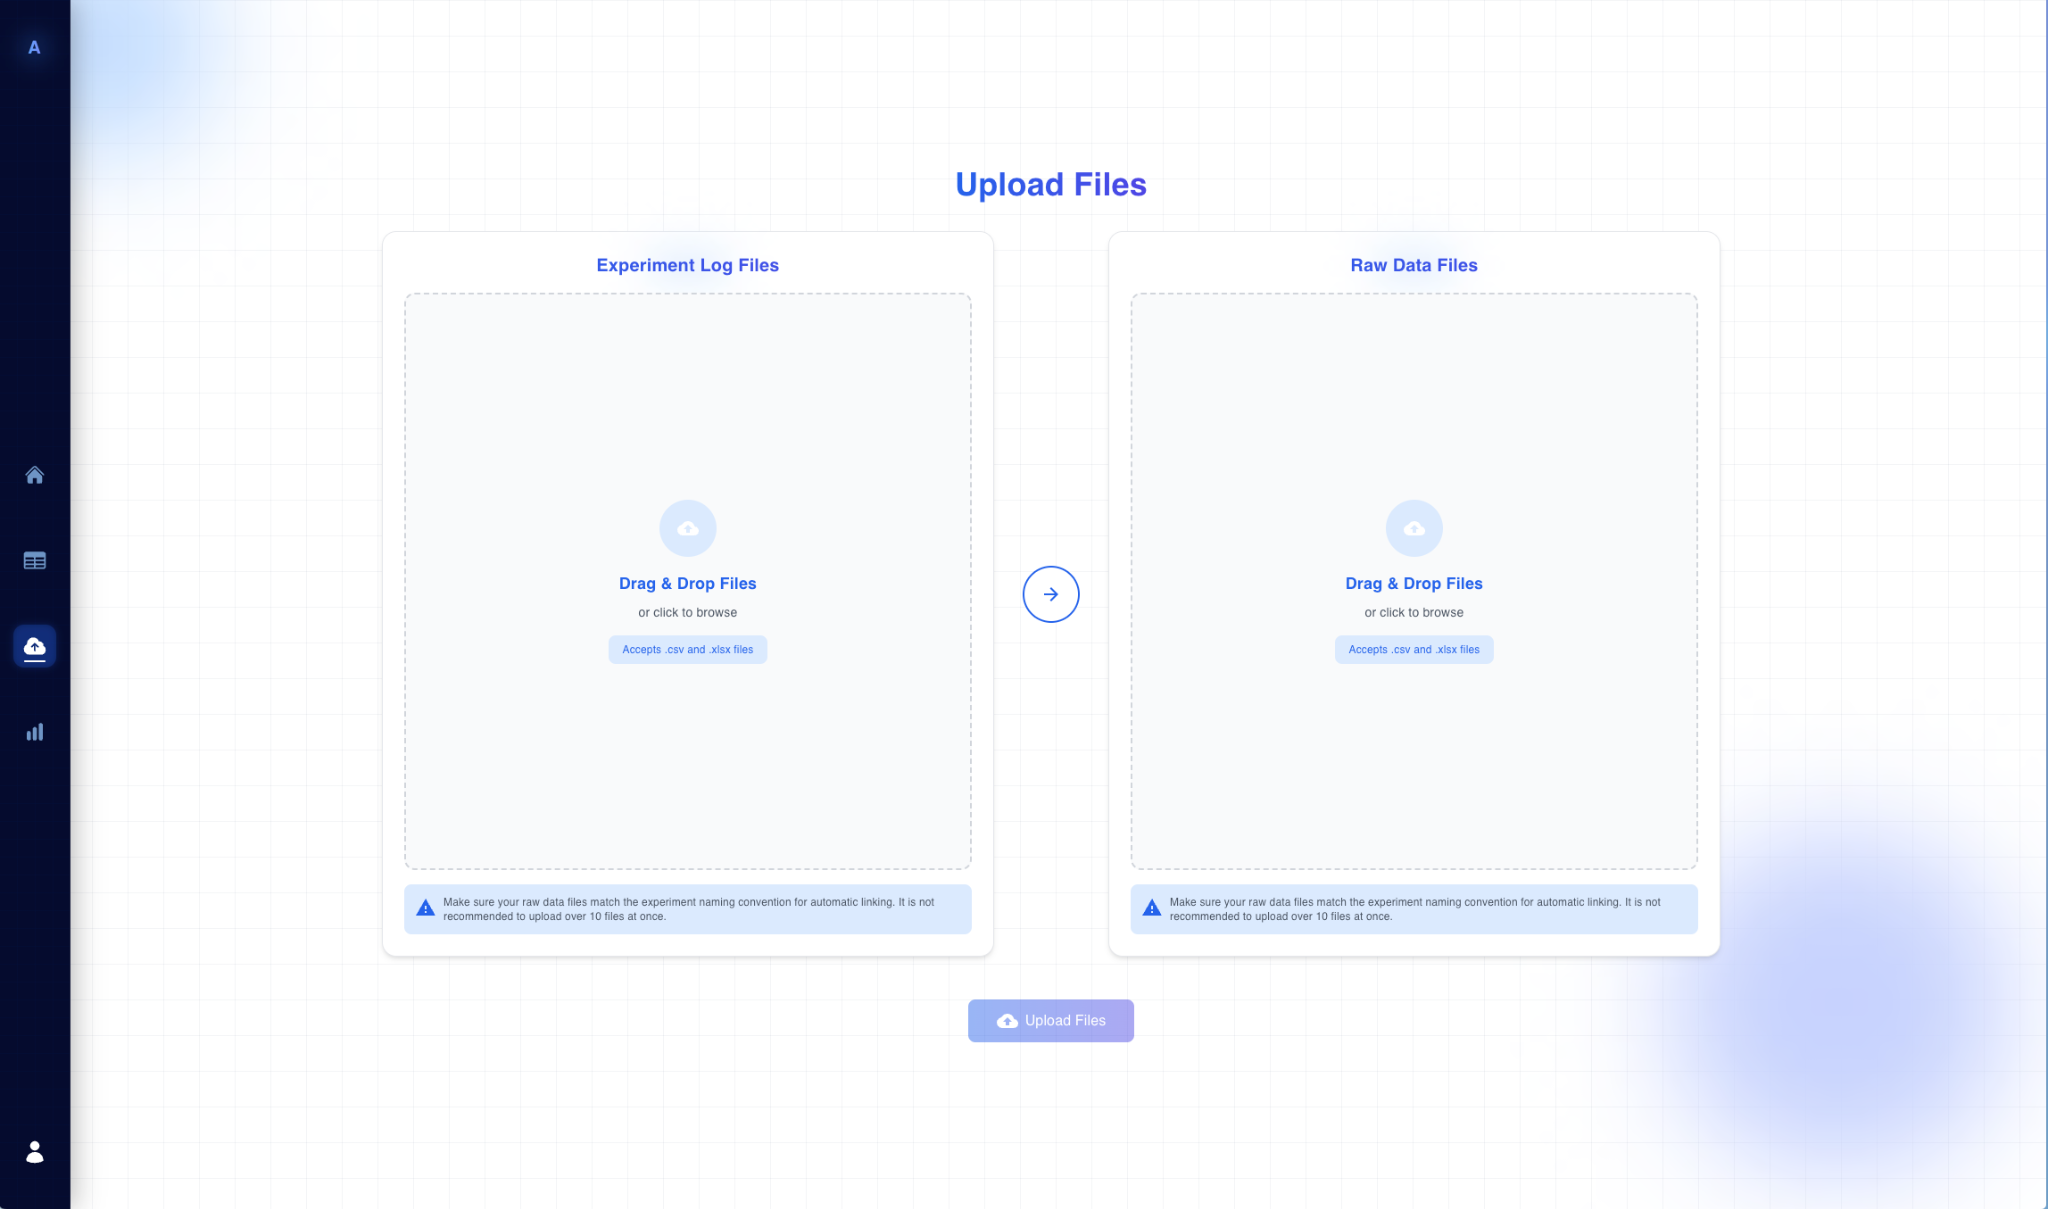
\includegraphics[width=0.8\textwidth]{./Diagrams/Upload.png}
    \caption{Upload Files Interface}
\end{figure}

\subsubsection{Step-by-Step Upload}
To upload files, follow these steps:
\begin{enumerate}
    \item Navigate to the Upload Page.
    \item Select the file type you wish to upload: either \textbf{Experiment
    Log} or \textbf{Raw Data}.
    \item Choose your preferred upload method:
    \begin{itemize}
        \item \textbf{Drag and Drop}: Drag files directly into the designated
        upload area.
        \item \textbf{Browse and Select}: Click on the upload box to open a file
        browser and select files manually.
    \end{itemize}
    \item Click the \textbf{Upload} button to initiate the upload process.
\end{enumerate}

\subsubsection{Linking Raw Data Files to Experiments}

In some cases, the migration algorithm may not be able to automatically link a
raw data file to its corresponding experiment. When this occurs, users will be
prompted to manually match the data file with the appropriate experiment ID.

\begin{figure}[H]
    \centering
    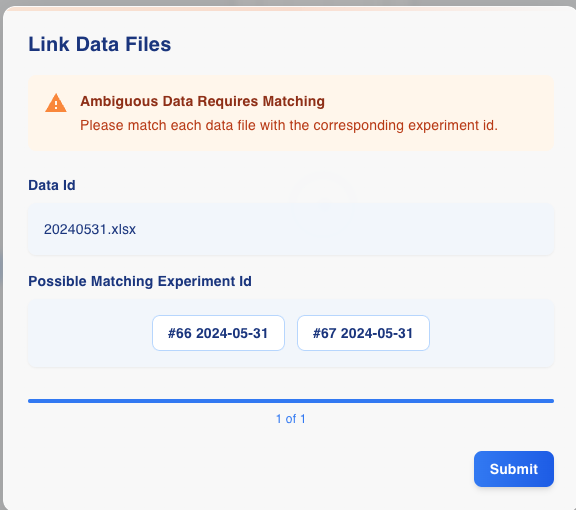
\includegraphics[width=0.8\textwidth]{./Diagrams/DataLinkModal.png}
    \caption{Link Data Files Prompt}
\end{figure}

When presented with this prompt, users should:

\begin{enumerate}
    \item Review the displayed Data ID to ensure it corresponds to the correct
    file.
    \item Select the appropriate Experiment ID from the provided options.
    \item Click the \textbf{Submit} button to confirm the link.
\end{enumerate}

This manual linking process ensures that all data files are accurately
associated with their respective experiments, maintaining data integrity and
facilitating effective analysis.

\subsubsection{File Requirements}
To ensure successful uploads, please adhere to the following file requirements:
\begin{table}[H]
    \centering
    \begin{tabularx}{\textwidth}{lX}
        \toprule
        \textbf{Requirement} & \textbf{Specification} \\
        \midrule
        File Size & Maximum 10MB per file \\
        Date Format & YYYY-MM-DD \\
        Special Characters & Avoid at all costs \\
        \bottomrule
    \end{tabularx}
\end{table}

\subsubsection{File Upload Types}
The upload interface categorizes files into two primary types to facilitate
structured data management:
\begin{itemize}
    \item \textbf{Experiment Log Files}: Processed logs containing IDs, dates,
    and input parameters.
    \item \textbf{Raw Data Files}: Experimental data outputted by the machine,
    including IDs, dates, and results.
\end{itemize}

\subsubsection{Supported File Formats}
The following file formats are supported for upload:
\begin{itemize}
    \item \textbf{CSV (.csv)}: A structured data format using comma-separated
    values.
    \item \textbf{Excel (.xlsx)}: A spreadsheet format that supports multiple
    sheets and structured data.
\end{itemize}

\subsubsection{Upload Guidelines}
To maintain system performance and ensure proper data processing, users should
follow these best practices:
\begin{itemize}
    \item Limit uploads to a maximum of 10 files at once.
    \item Ensure that data structures match the expected formats to prevent
    processing errors.
    \item If a file does not meet the required format, the system may issue a
    warning or reject the upload.
\end{itemize}


\subsection{Data View}

The Data View section provides users with a structured and interactive way to
explore the data uploaded into the system. 

\subsubsection{Common Functionalities}
Across all tables, users can utilize the following common functionalities to
enhance their data exploration experience:
\begin{itemize}
    \item \textbf{Search}: Locate specific data points quickly using the dynamic
    search bar. Users can search across the entire dataset or within a single
    column by selecting the desired field from the dropdown menu.
    \item \textbf{Sorting}: Organize data systematically by clicking on any
    column header to sort entries in ascending or descending order. Sorting
    indicators (arrows) will reflect the current order.
    \item \textbf{Highlighting Matches}: Relevant data points are automatically
    highlighted upon search, drawing immediate attention to key results.
    \item \textbf{Row Filtering}: Non-matching rows are temporarily removed from
    view, simplifying the focus on pertinent data.
    \item \textbf{Column Navigation}: Each column is labeled alphabetically (A,
    B, C, etc.) for easy reference, ensuring that users can quickly identify and
    focus on specific data fields.
\end{itemize}

\subsubsection{Experiment Table}
The Experiment Table  provides comprehensive oversight of all experiment-related
data. This table allows full control over data management, including editing and
deleting entries, making it an essential tool for maintaining data accuracy and
integrity.

\begin{figure}[H]
    \centering
    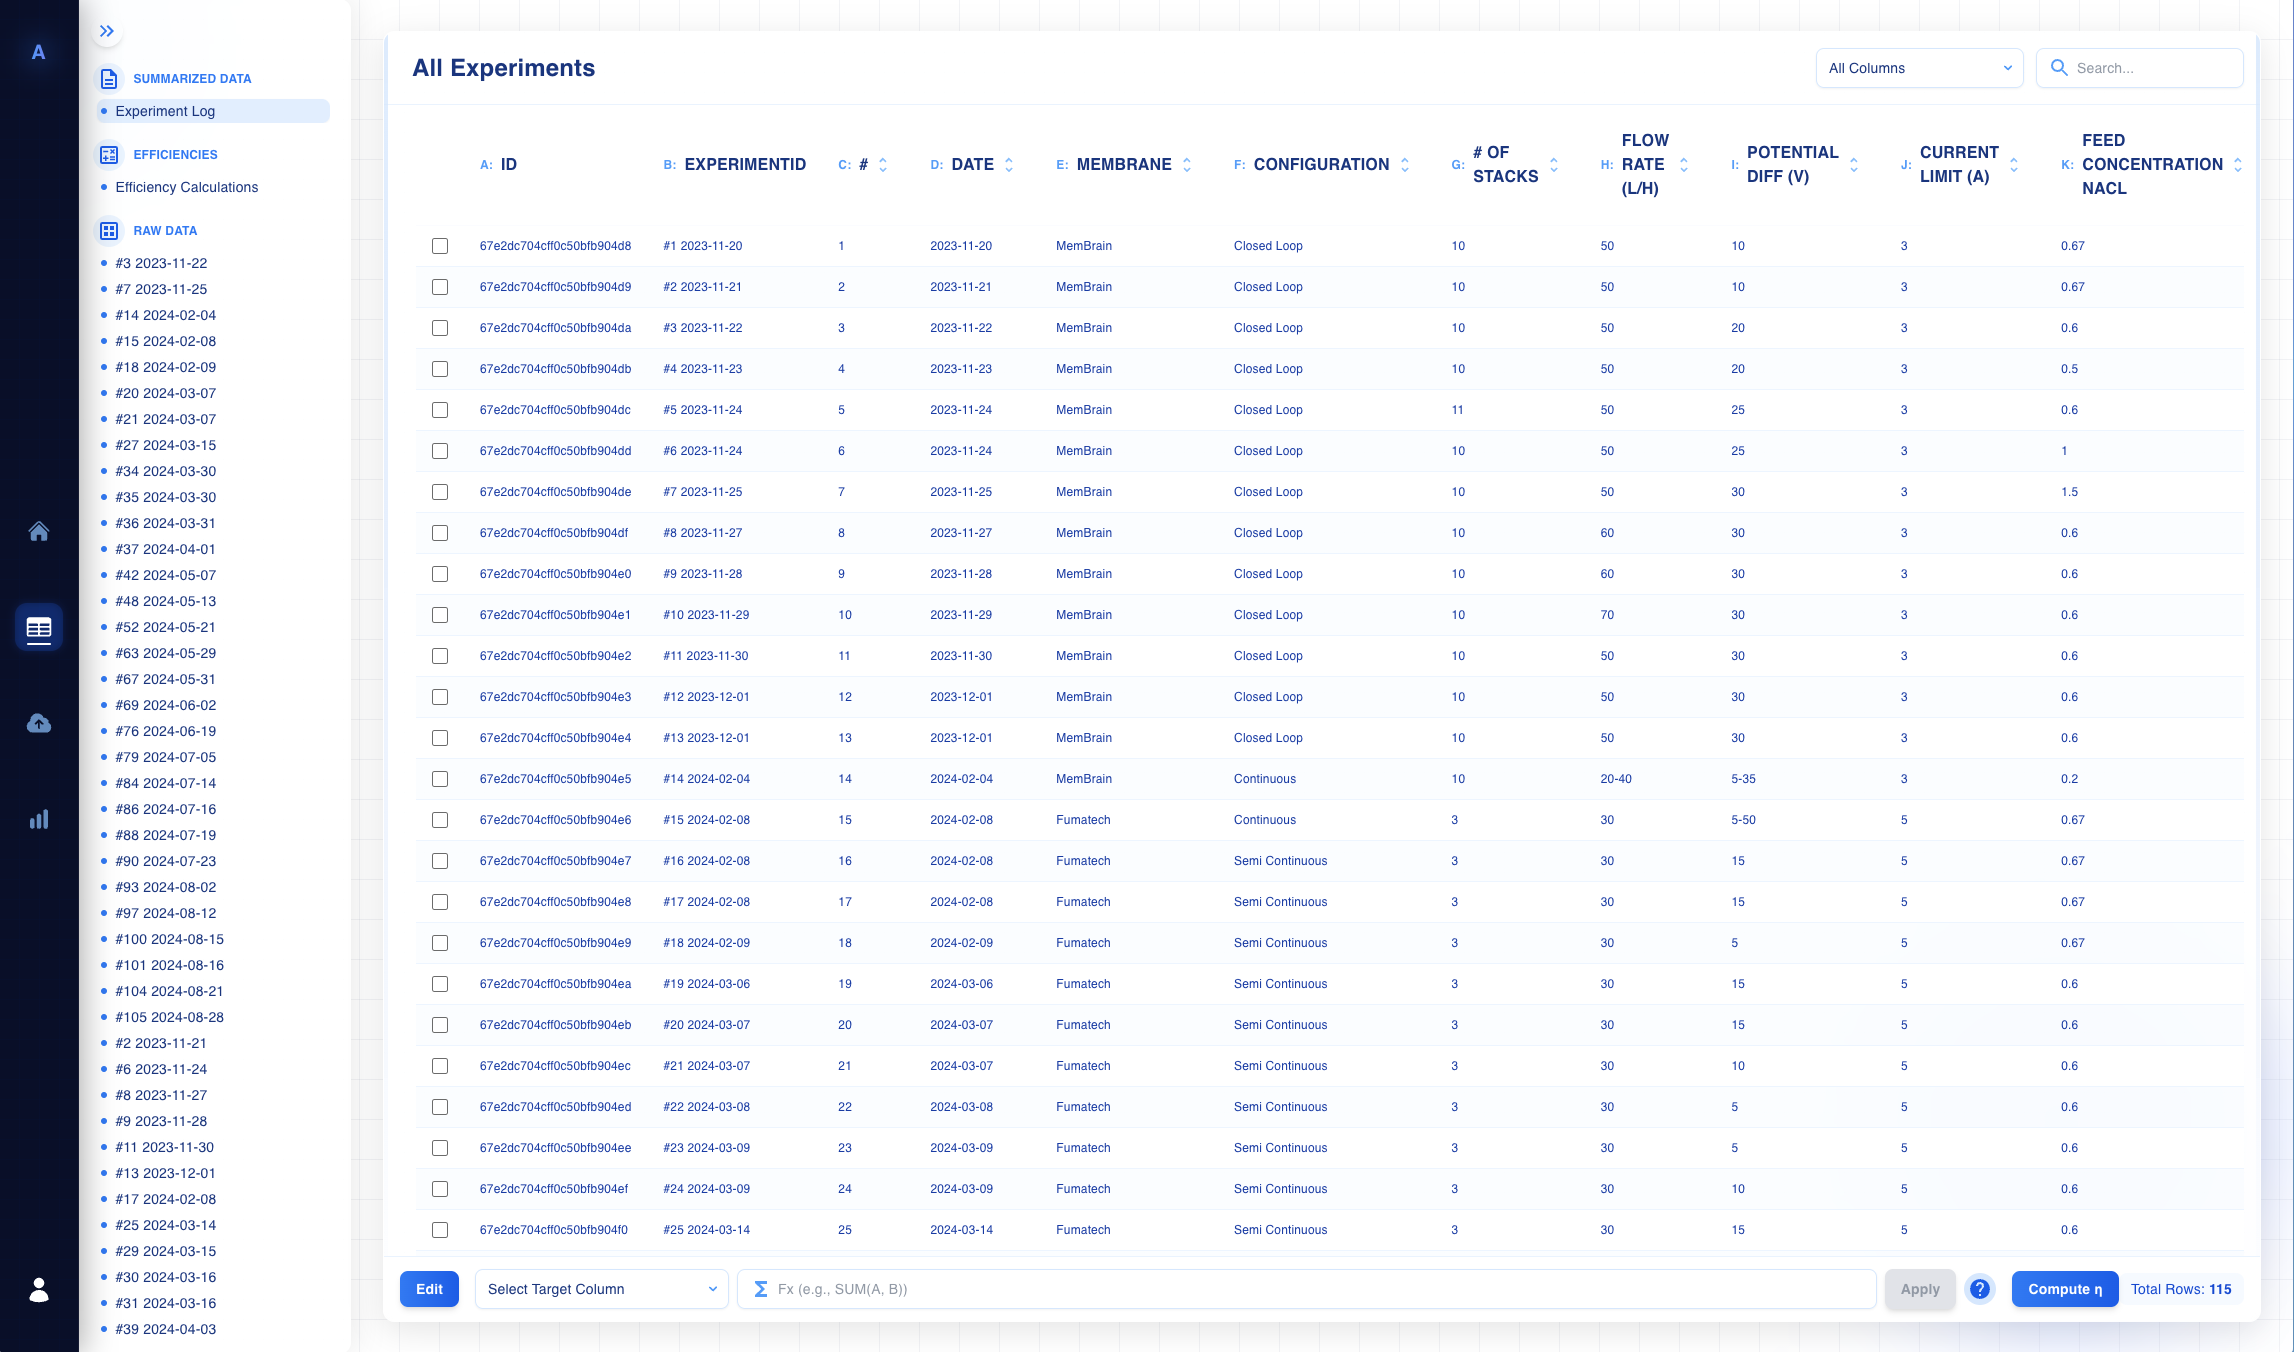
\includegraphics[width=0.8\textwidth]{./Diagrams/ExperimentTableView.png}
    \caption{Experiment Table View}
\end{figure}

\paragraph{Row Selection}
The Row Selection feature allows users to select one or more rows for bulk
actions such as editing or deleting.
\begin{enumerate}
    \item Click the checkbox next to each row you wish to select.
    \item Perform the desired bulk action (e.g., editing or deleting) on the
    selected rows.
\end{enumerate}

\paragraph{Edit Dropdown Menu}
The Edit Dropdown Menu enables users to edit the table directly.
\begin{enumerate}
    \item Click the "Edit" button to view available options.
    \item Select the desired option from the dropdown menu.
\end{enumerate}

\paragraph{Add Column}
The Add Column feature allows users to introduce a new column into the table for
additional data entry.
\begin{enumerate}
    \item Click the "Add Column" button.
    \item Enter a name for the new column in the dialog box that appears.
    \item The new column will be added to the right side of the table.
\end{enumerate}

\begin{figure}[H]
    \centering
    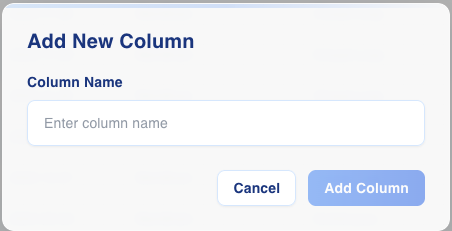
\includegraphics[width=0.6\textwidth]{./Diagrams/AddColumn.png}
    \caption{Add New Column Dialog}
\end{figure}

\paragraph{Add Row}
The Add Row feature enables users to insert a new row into the table for
additional data entries.
\begin{enumerate}
    \item Click the "Add Row" button.
    \item A form will appear, prompting you to enter values for each column.
    \item Fill in the required fields and click "Submit" to add the new row.
\end{enumerate}

\begin{figure}[H]
    \centering
    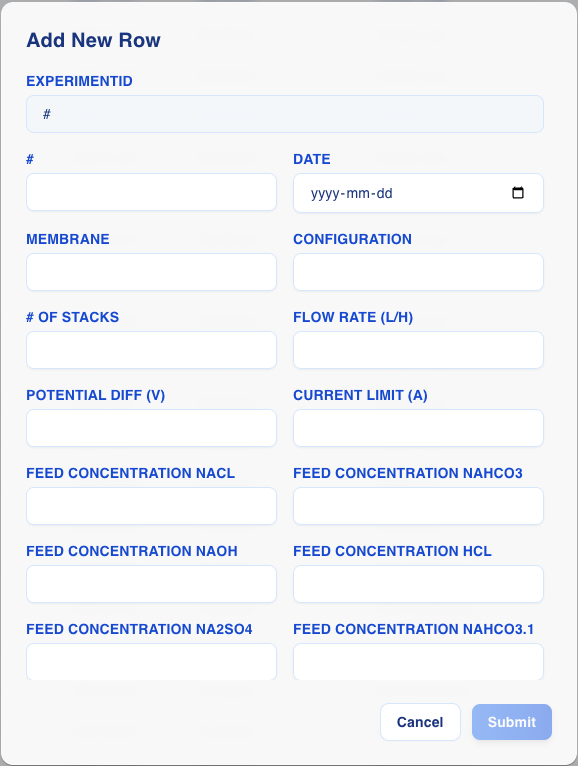
\includegraphics[width=0.6\textwidth]{./Diagrams/AddRow.png}
    \caption{Add New Row Dialog}
\end{figure}

\paragraph{Remove Column}
The Remove Column feature allows users to delete an existing column from the
table.
\begin{enumerate}
    \item Click the "Remove Column" button.
    \item Select the column you wish to remove from the dropdown menu.
    \item Confirm your action by clicking "Remove Column." 
    \item Note that this operation cannot be undone.
\end{enumerate}

\begin{figure}[H]
    \centering
    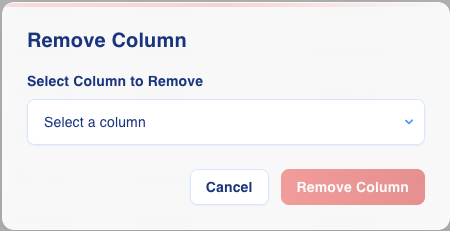
\includegraphics[width=0.6\textwidth]{./Diagrams/RemoveColumn.png}
    \caption{Remove Column Dialog}
\end{figure}

\paragraph{Remove Row}
The Remove Row feature enables users to delete one or more selected rows from
the table.
\begin{enumerate}
    \item Select one or more rows by checking the boxes next to them.
    \item Click the "Remove Column" button.
    \item Click the "Remove Row" button to open a confirmation dialog.
    \item Review the warning message and click "Remove Row" again to delete the
    selected rows permanently.
\end{enumerate}

\begin{figure}[H]
    \centering
    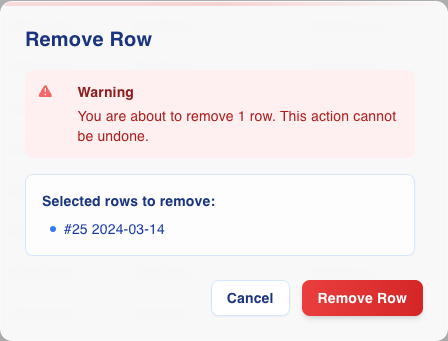
\includegraphics[width=0.6\textwidth]{./Diagrams/RemoveRowWithSelectedRow.png}
    \caption{Remove Row Confirmation Dialog}
\end{figure}

\paragraph{Set Column Types}
The Set Column Types feature allows administrators to define the data type for
each column in the table, ensuring consistency and accuracy.
\begin{enumerate}
    \item Navigate to the "Set Column Types" section.
    \item Select the desired data type (e.g., Number, Date, Text) for each
    column from the dropdown menu.
    \item Click "Save Changes" to apply the updates.
\end{enumerate}

\begin{figure}[H]
    \centering
    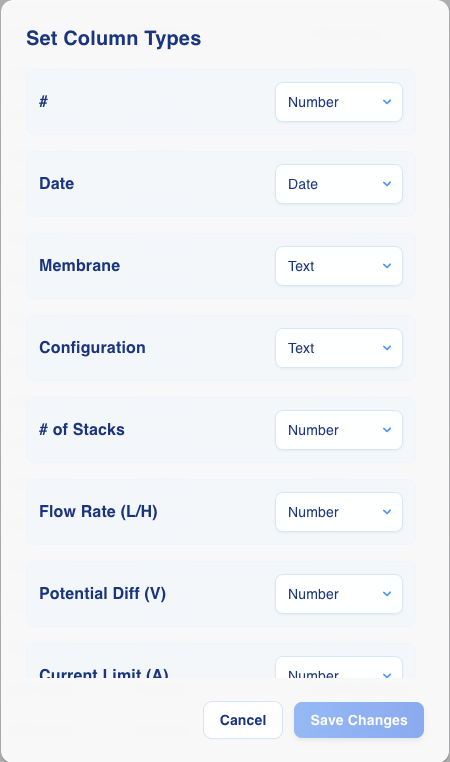
\includegraphics[width=0.5\textwidth]{./Diagrams/SetColumnType.png}
    \caption{Set Column Types Dialog}
\end{figure}

\paragraph{Function Bar}
The Function Bar at the bottom of the table enables advanced data manipulation
through calculations.
\begin{enumerate}
    \item Select the rows you want to include in the calculation by checking the
    boxes next to them.
    \item Choose the target column where the calculated result will be applied.
    \item Enter a formula using column headers (e.g., SUM(G, I)).
    \item Click the "Apply" button to calculate and update the target column
    with the results.
\end{enumerate}


\begin{figure}[H]
    \centering
    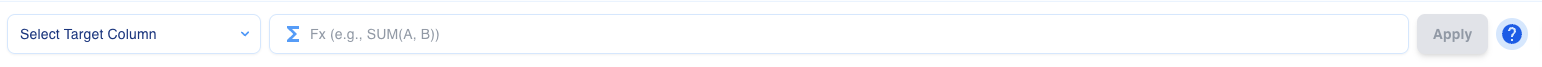
\includegraphics[width=1\textwidth]{./Diagrams/FunctionBar.png}
    \caption{Function Bar}
\end{figure}

\paragraph{Compute Efficiency Factors}
The Compute Efficiency Factors tool enables administrators to calculate various
efficiency metrics based on selected experiments and time intervals.
\begin{enumerate}
    \item Click the "Compute $\eta$" button.
    \item Select an experiment for which you want to compute efficiency factors.
    \item Define the duration over which the calculations will be performed.
    \item Select Efficiency Factor to compute.
\end{enumerate}

\begin{figure}[H]
    \centering
    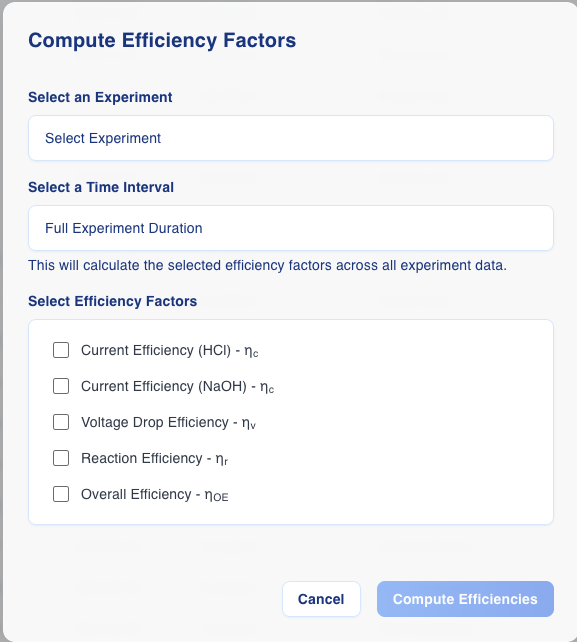
\includegraphics[width=0.6\textwidth]{./Diagrams/ComputeEffFactors.png}
    \caption{Compute Efficiency Factors Dialog}
\end{figure}

\subsubsection{Efficiency Table (Read-Only)}
The Efficiency Table offers a read-only view of efficiency metrics derived from
the processed data. This table is designed to provide insights into performance
trends and outcomes, enabling users to understand the effectiveness of their
experiments without the ability to modify the underlying data.

\subsubsection{Raw Data Table (Read-Only)}
The Raw Data Table presents a read-only view of the raw experimental data,
offering users the ability to explore detailed information captured during
experiments. This table is crucial for users who need to examine individual data
points and verify the integrity of the uploaded information without altering it.

% \begin{figure}[H] \centering
%     \includegraphics[width=0.8\textwidth]{./Diagrams/RawDataTable.png}
%     \caption{Raw Data Table View} \end{figure}

\subsection{Graph Generation}

This section provides detailed instructions for creating, customizing, and
exporting data visualizations.

\subsection*{Page Overview}
The graph page is seperated in two sections. 
\newline \newline
\textbf{Side Bar:} \newline
On the left side of the page is the sidebar where it displays all the recently
generated graphs and has the generate new graph button.
\newline\newline

\noindent \textbf{Main Content:}\newline
On the right is the main content of the page. Here, the generated graph will be
displayed along with a quick linear regression analysis with a short statement
of its findings 
\begin{figure}[H]
    \centering
    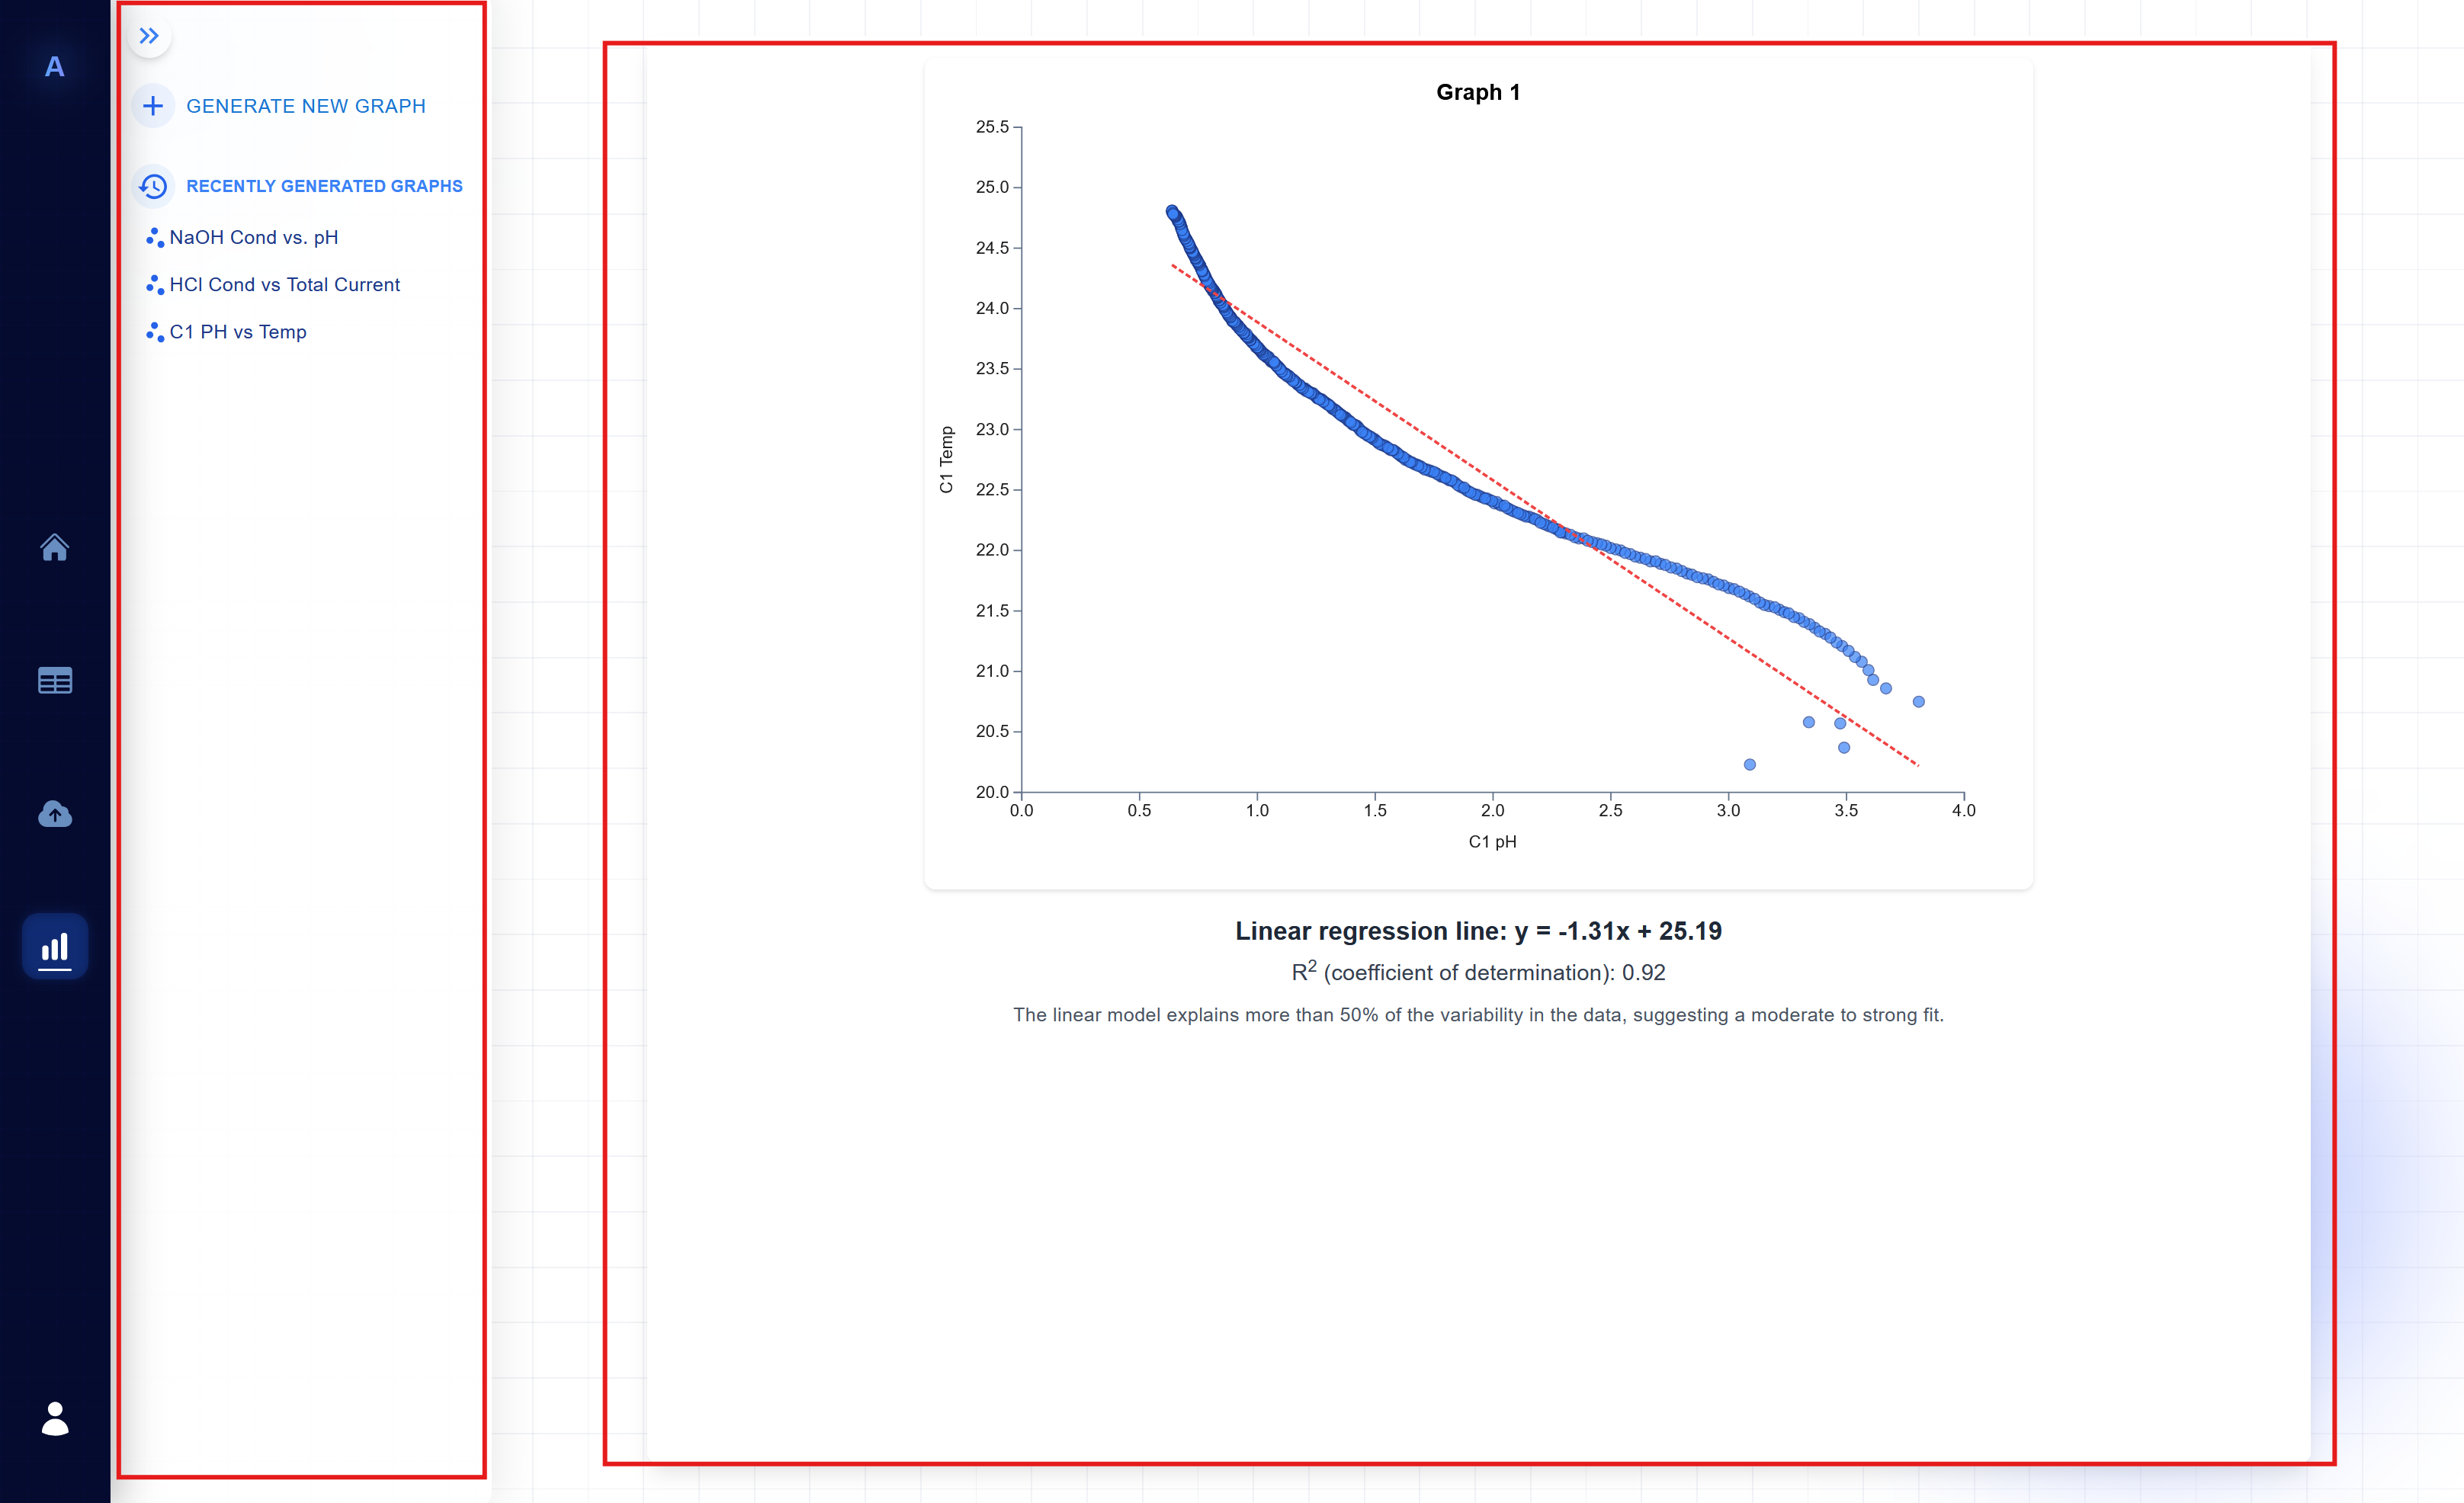
\includegraphics[scale=0.3]{Images/graph page .png}
    \caption{Graph page Seperation Display}
    \label{fig:example}
\end{figure}

On the side bar, beside each generated graph item has an icon which signifies
the type of graph it is. 
\begin{table}[H]
    \centering
    \begin{tabular}{|c|c|}
        \hline
         \textbf{Icon} & \textbf{Definition} \\
        \hline
        
\includegraphics[width=1.5cm]{Images/graph-line.png} & Line Graph \\
        \hline
        
\includegraphics[width=1.5cm]{Images/graph-bar.png} & Bar Graph \\
        \hline
        
\includegraphics[width=1.5cm]{Images/graph-scatter.png} & Scatter Plot \\
        \hline
    \end{tabular}
    \caption{Graph Types and Their Definitions}
    \label{tab:graphs}
\end{table}

\noindent \textbf{Generting a New Graph:} \newline
To create a new graph, click on the \textbf{Generate New Graph} button at the top of the side bar:
\begin{figure}[H]
    \centering
    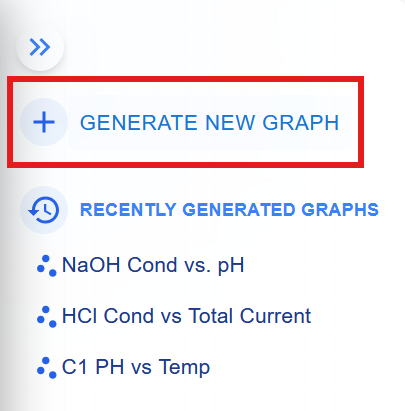
\includegraphics[scale=1]{Images/graph-newgraph .png}
    \caption{Highlights the Generate New Graph Button}
    \label{fig:example}
\end{figure}
\subsubsection{Detailed Workflow}
\subsubsection*{Description}
There is a five-step process for generating custom graphs from experimental data.

\begin{enumerate}
    \item \textbf{Select Graph Type:} \newline
    The app currently only supports 3 types of graphs. 
    \begin{itemize}
        \item Line graph 
        \item Bar graph 
        \item Scatter plot
    \end{itemize}
    \begin{figure}[H]
        \centering
        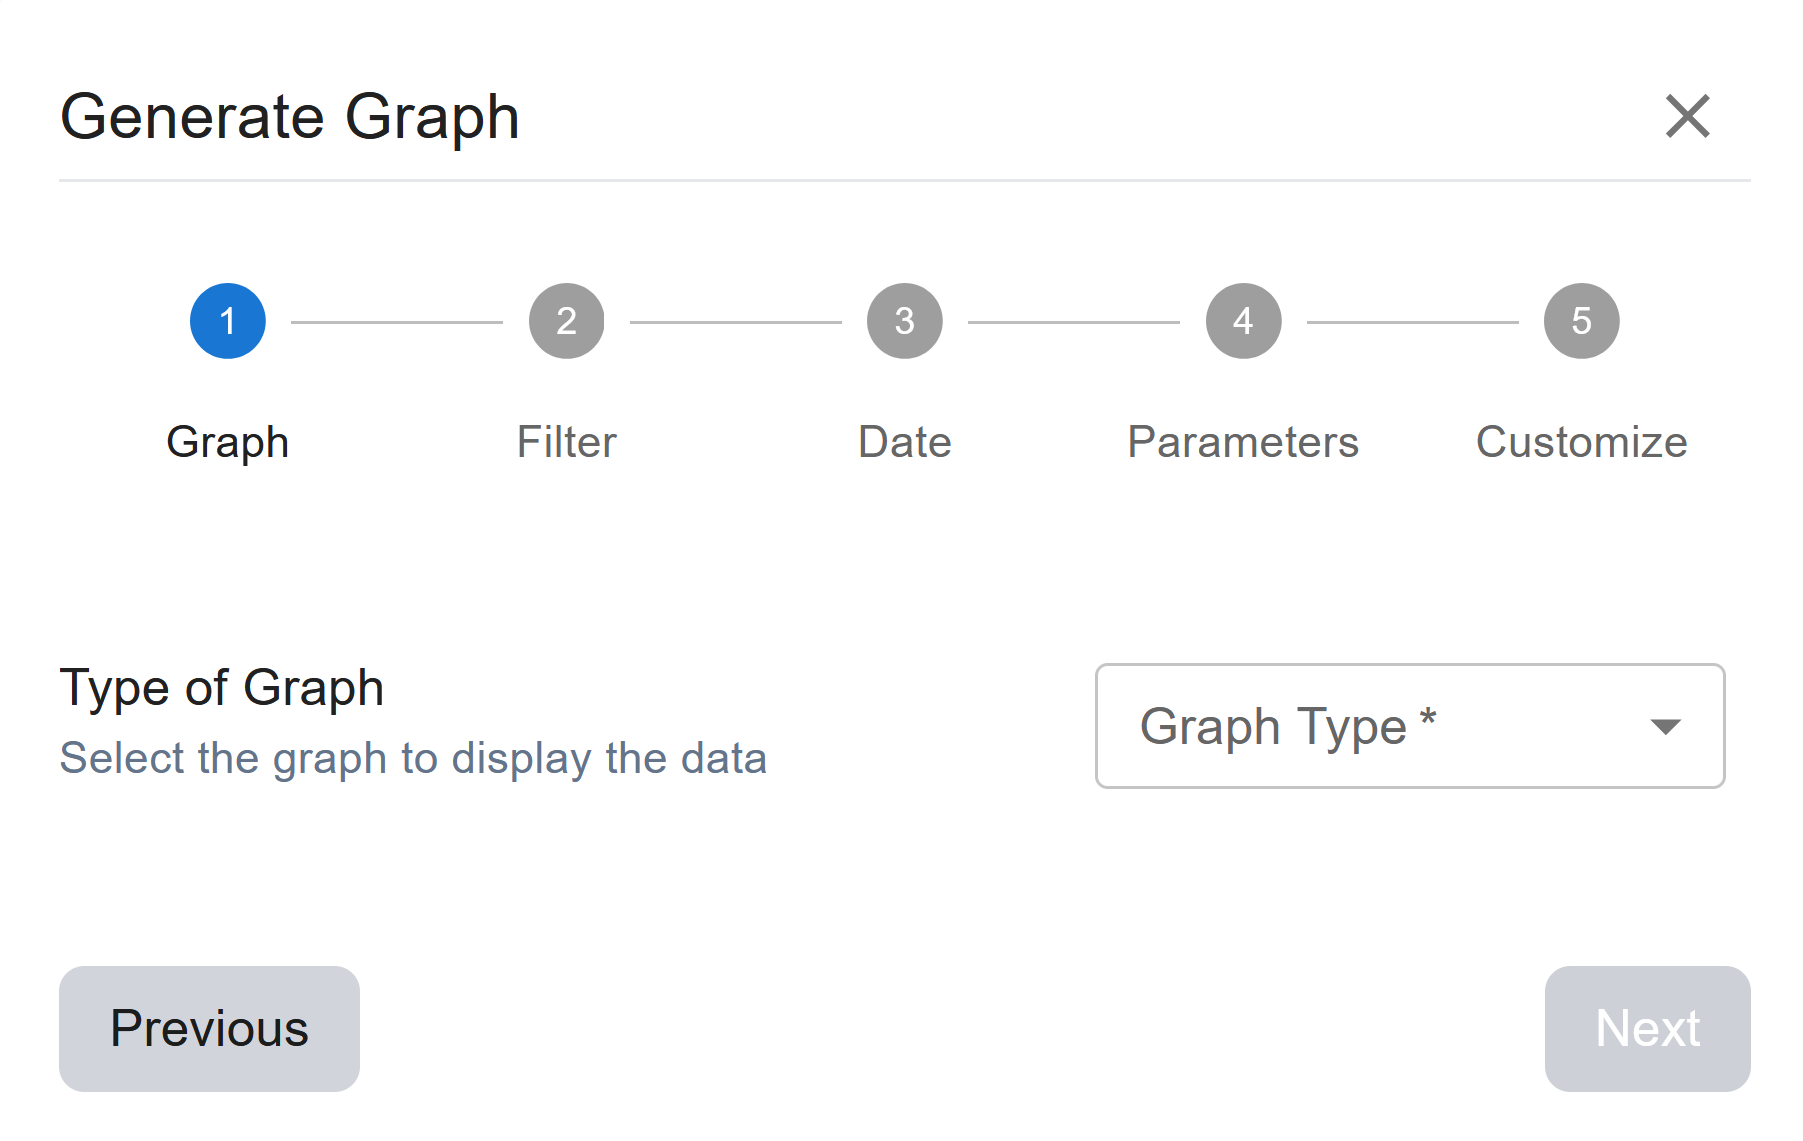
\includegraphics[scale=0.4]{Images/graph-form .png}
        \caption{Highlights the Generate New Graph Button}
        \label{fig:example}
    \end{figure}

    \item \textbf{Optional: Apply Filters}: \newline
    Use this part of the form to filter experiment dates based on a certain
    attribute. The attribute could be from the Experiment or Raw Data files.
    \newline
    \textbf{Note:} Either all form field must be willed out or all must be empty in order
    to progress to the next stage of the form. 
    \begin{enumerate}
        \item Choose which data file attribute to filter by
        \item Choose filter attribute 
        \item Select filter value from dropdown
    \end{enumerate}
    \begin{figure}[H]
        \centering
        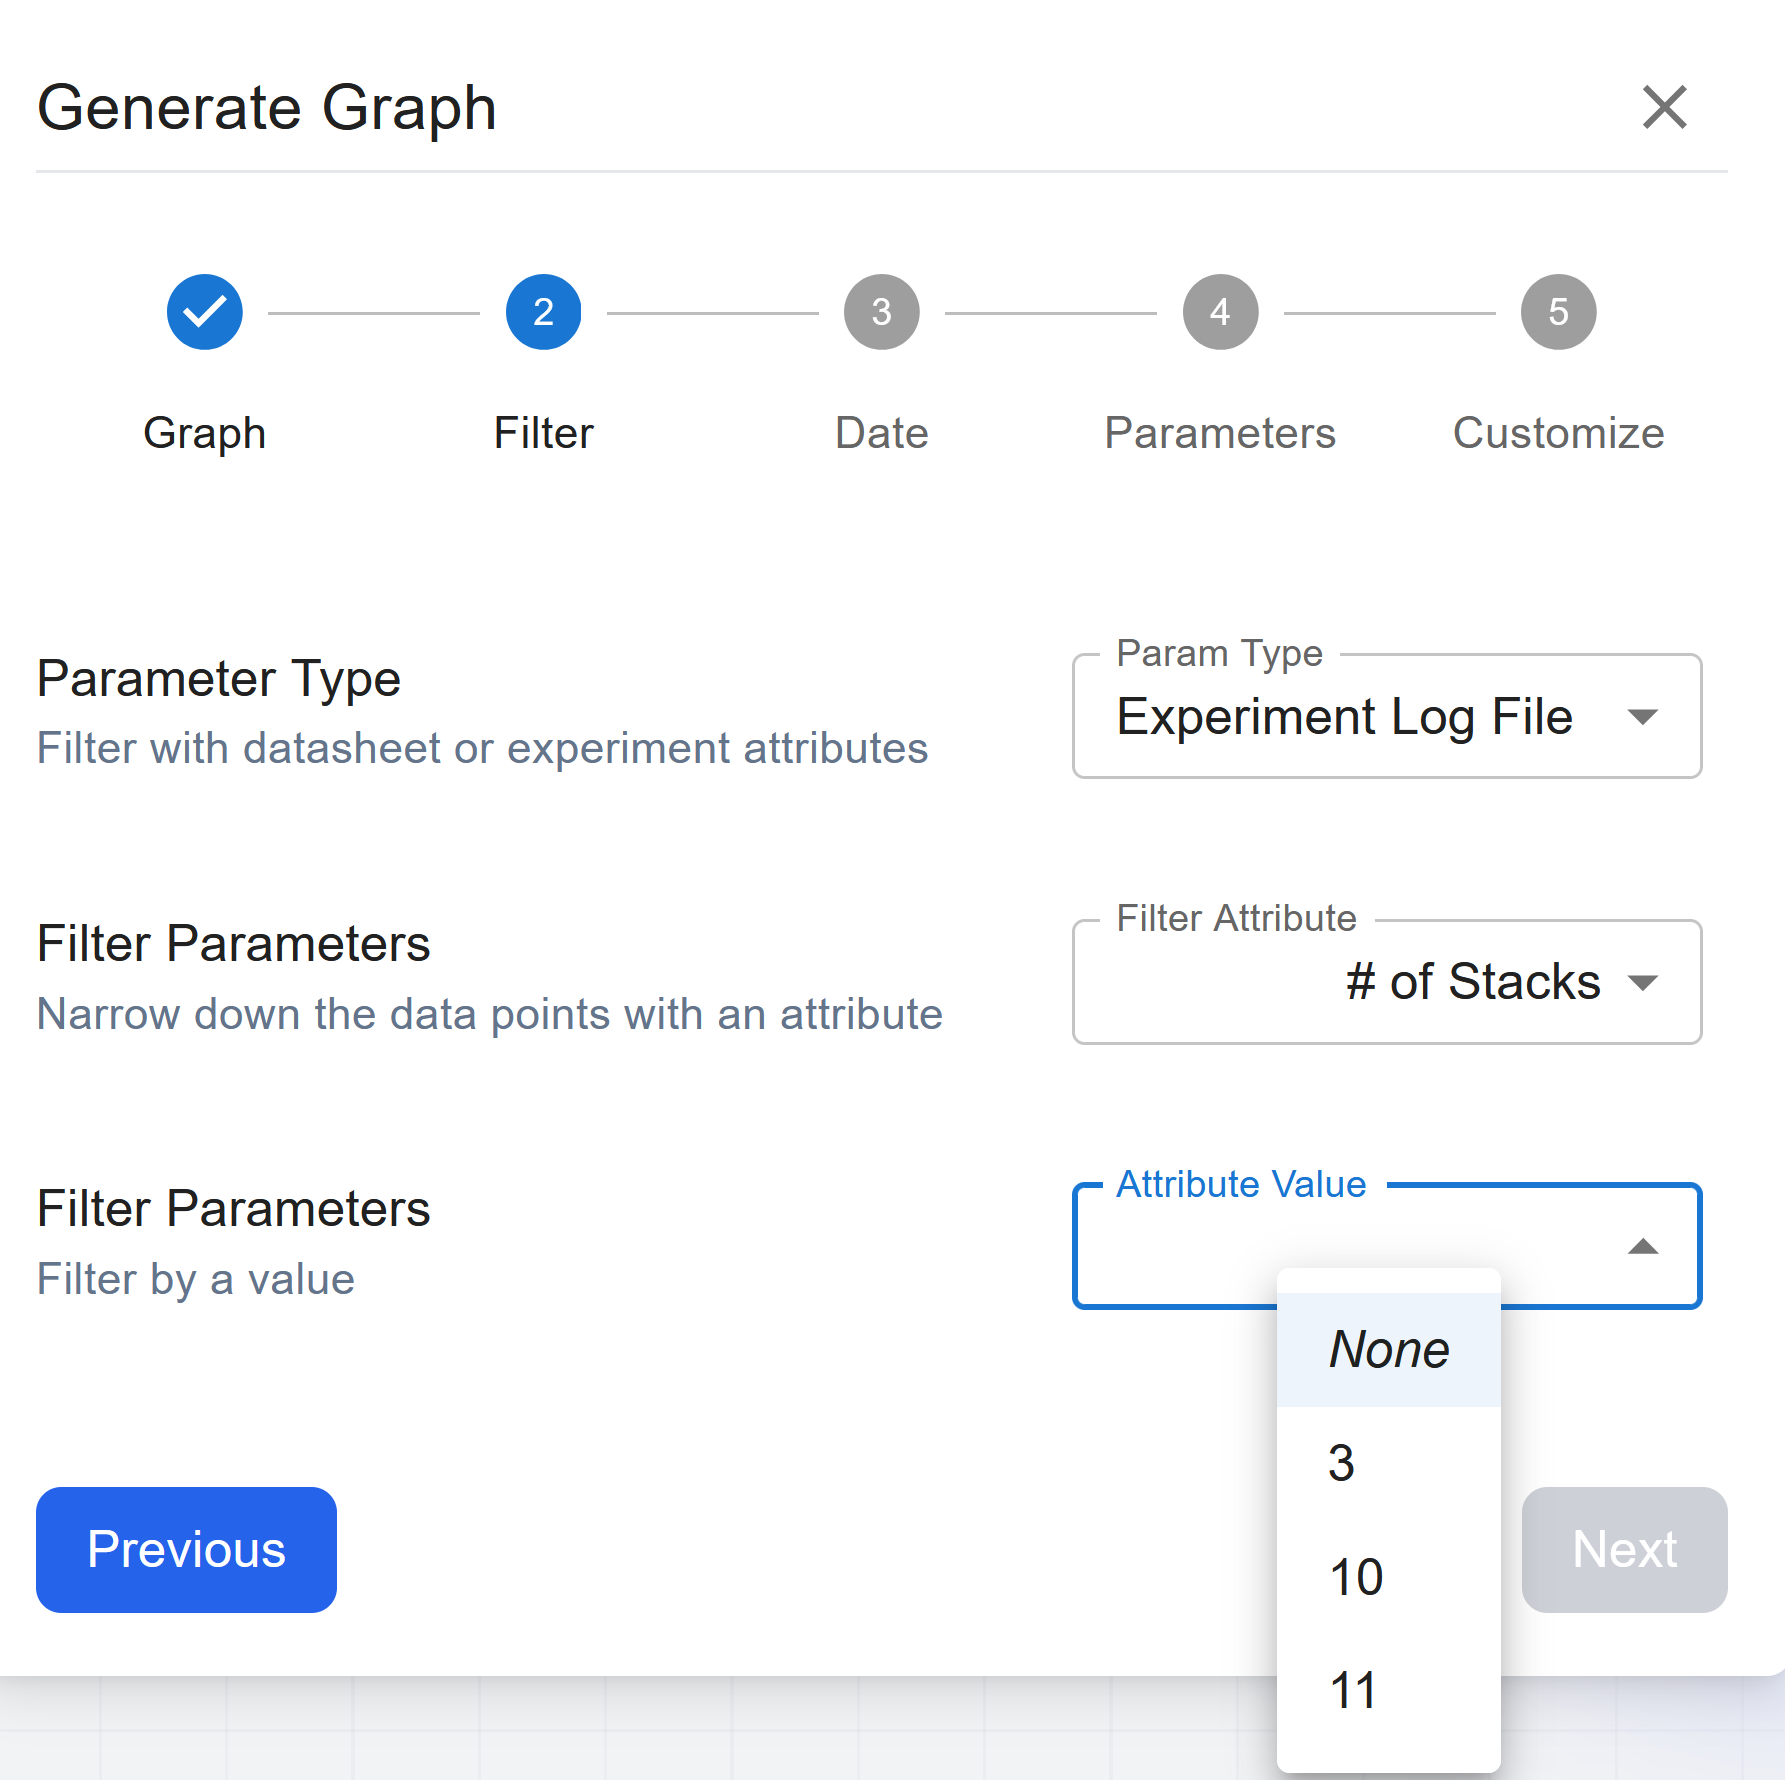
\includegraphics[scale=0.4]{Images/graph-filter.png}
        \caption{Sample Input of the Filter Step}
        \label{fig:example}
    \end{figure}

    \item \textbf{Selecting Dates}: \newline
    If no filter is applied, all experiemnt dates wil be listed. 
    \begin{figure}[H]
        \centering
        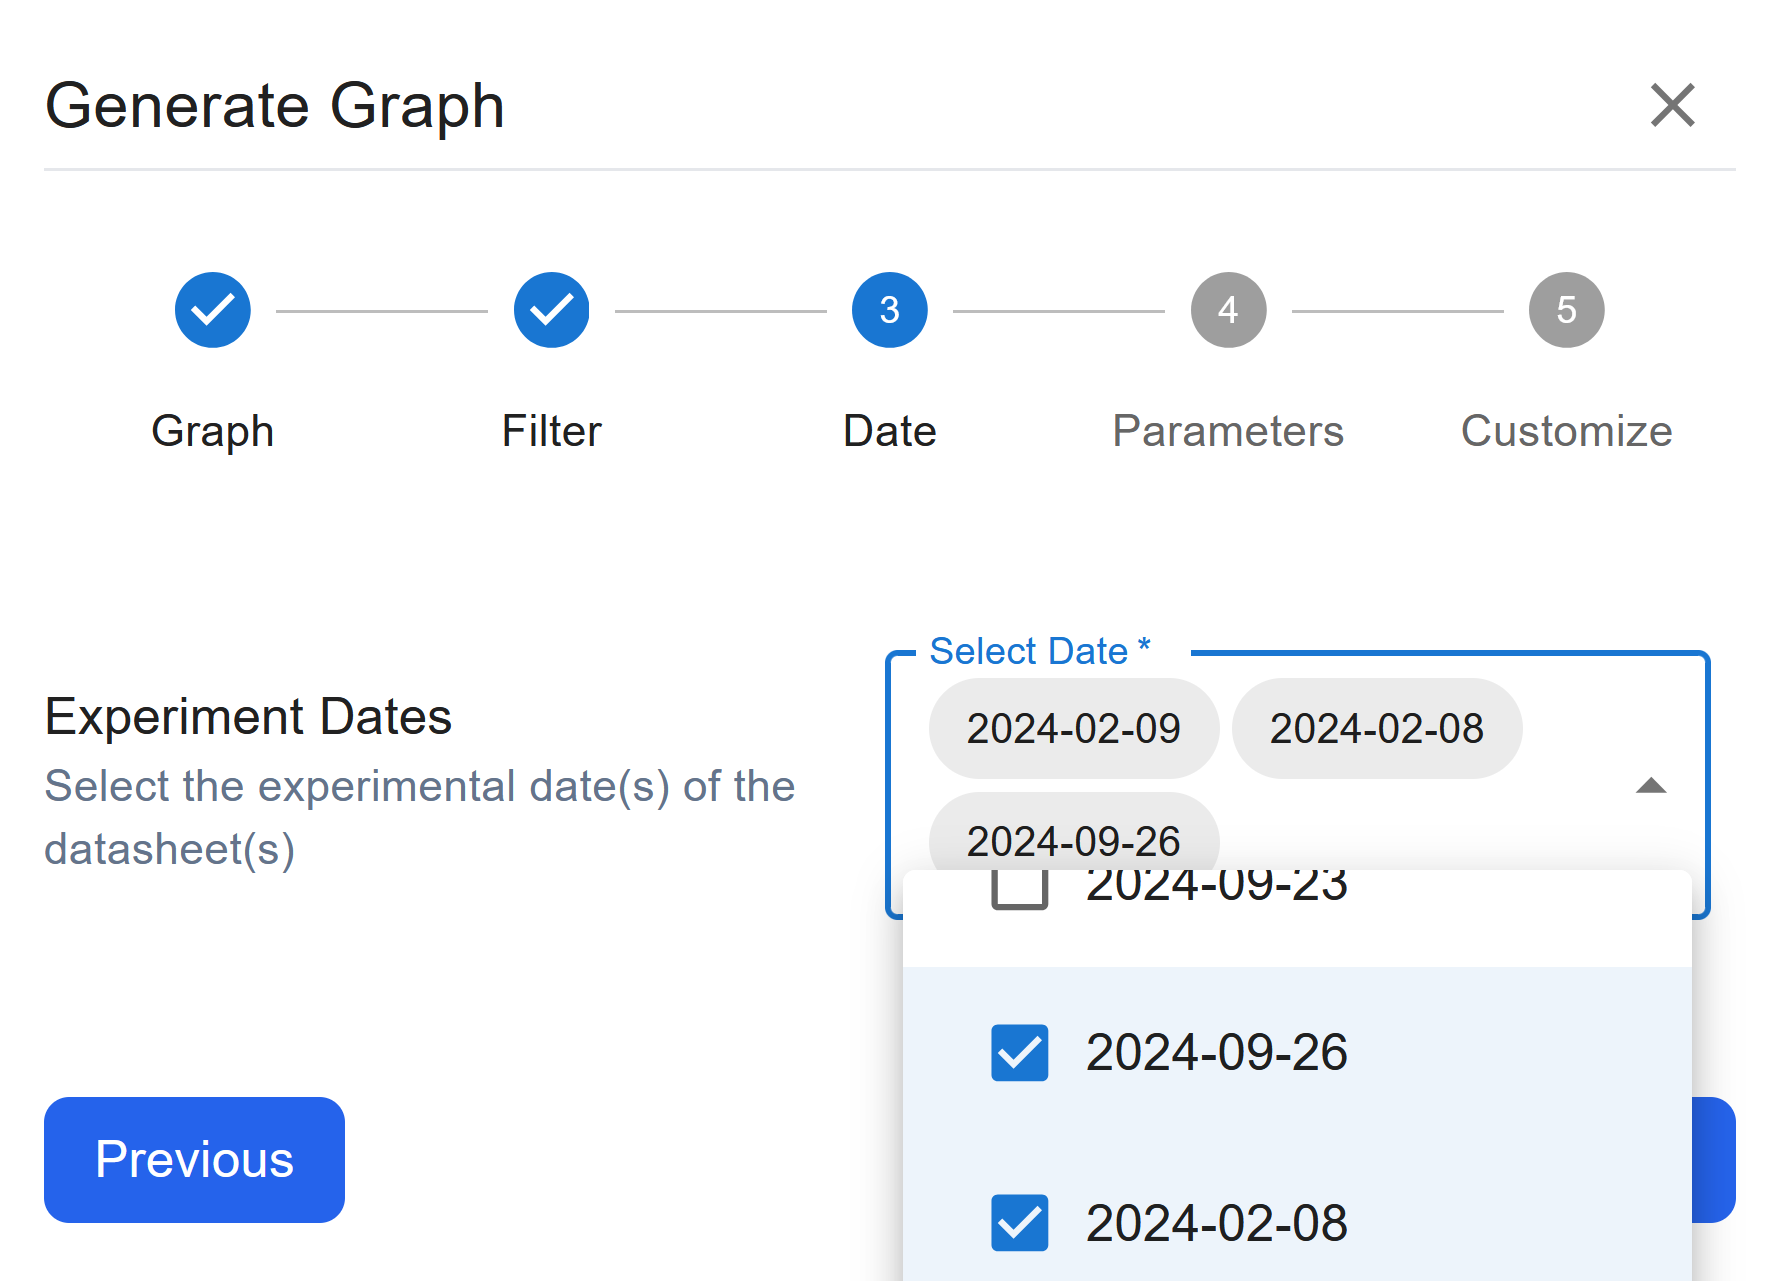
\includegraphics[scale=0.4]{Images/graph-dates.png}
        \caption{Sample Input of the Date Step}
        \label{fig:example}
    \end{figure}
    
    \item \textbf{Set Parameters}: \newline
    Select the attributes for the X and Y axis to plot. The two attributes must
    be from the same experiment sheet. 
    \begin{figure}[H]
        \centering
        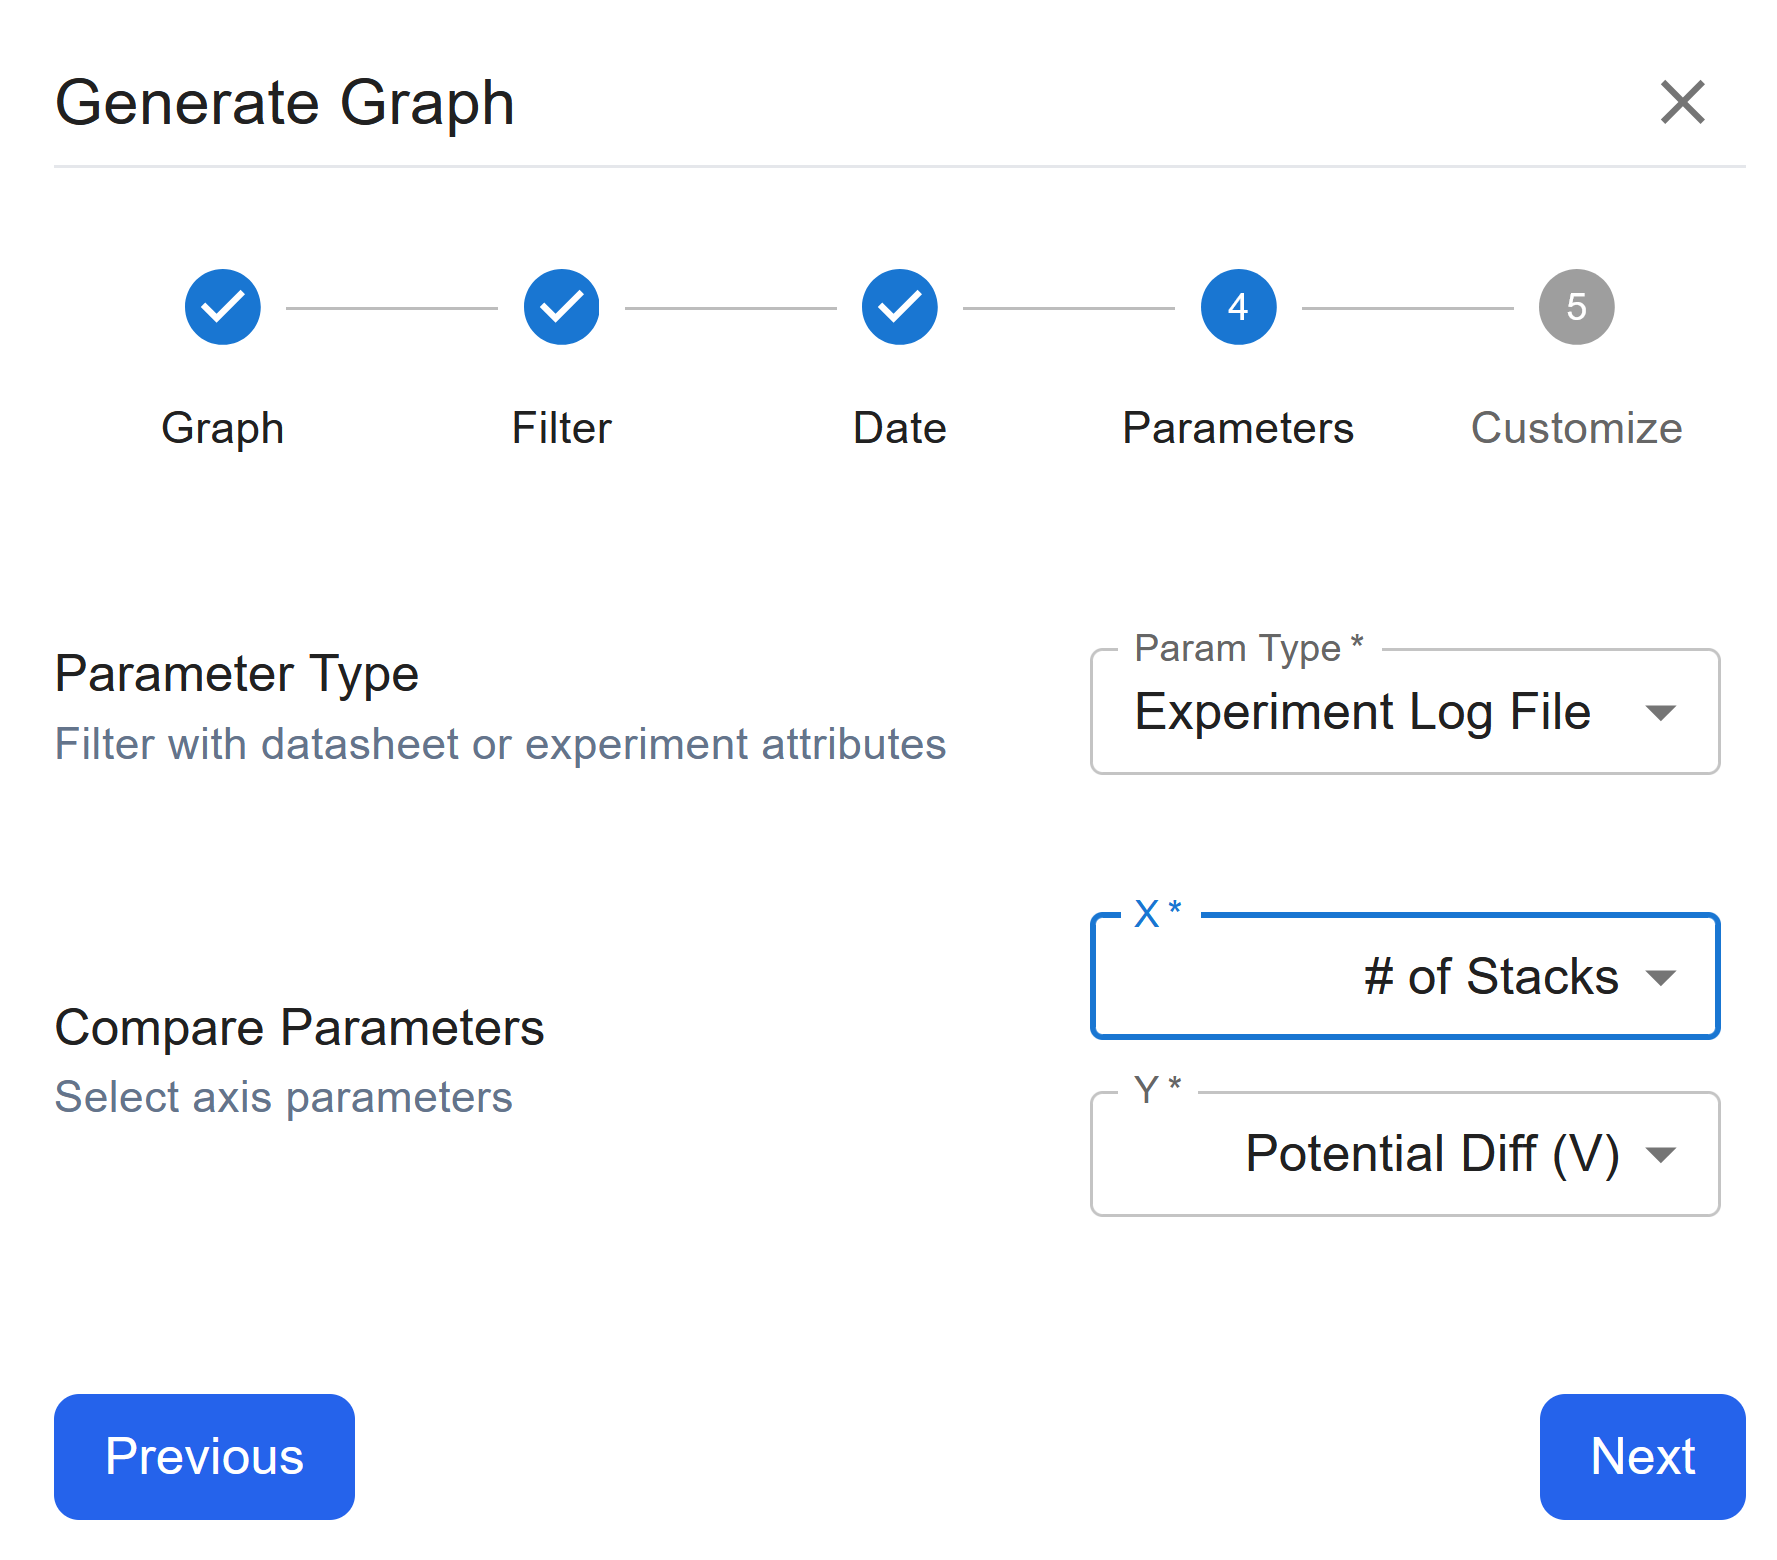
\includegraphics[scale=0.4]{Images/graph-param.png}
        \caption{Sample Input of the Filter Step}
        \label{fig:example}
    \end{figure}
    
    \item \textbf{Customize Display}: \newline
    Users are able to customize the graphs. All fields on this step are
    optional.If no axis labels are inputted, the axis would be nammed the
    attribute name selected by default.
    \newline
    There are the following options for customization
    \begin{itemize}
        \item Graph title
        \item Axis Ranges
        \item Axis Labels
    \end{itemize}
    \begin{figure}[H]
        \centering
        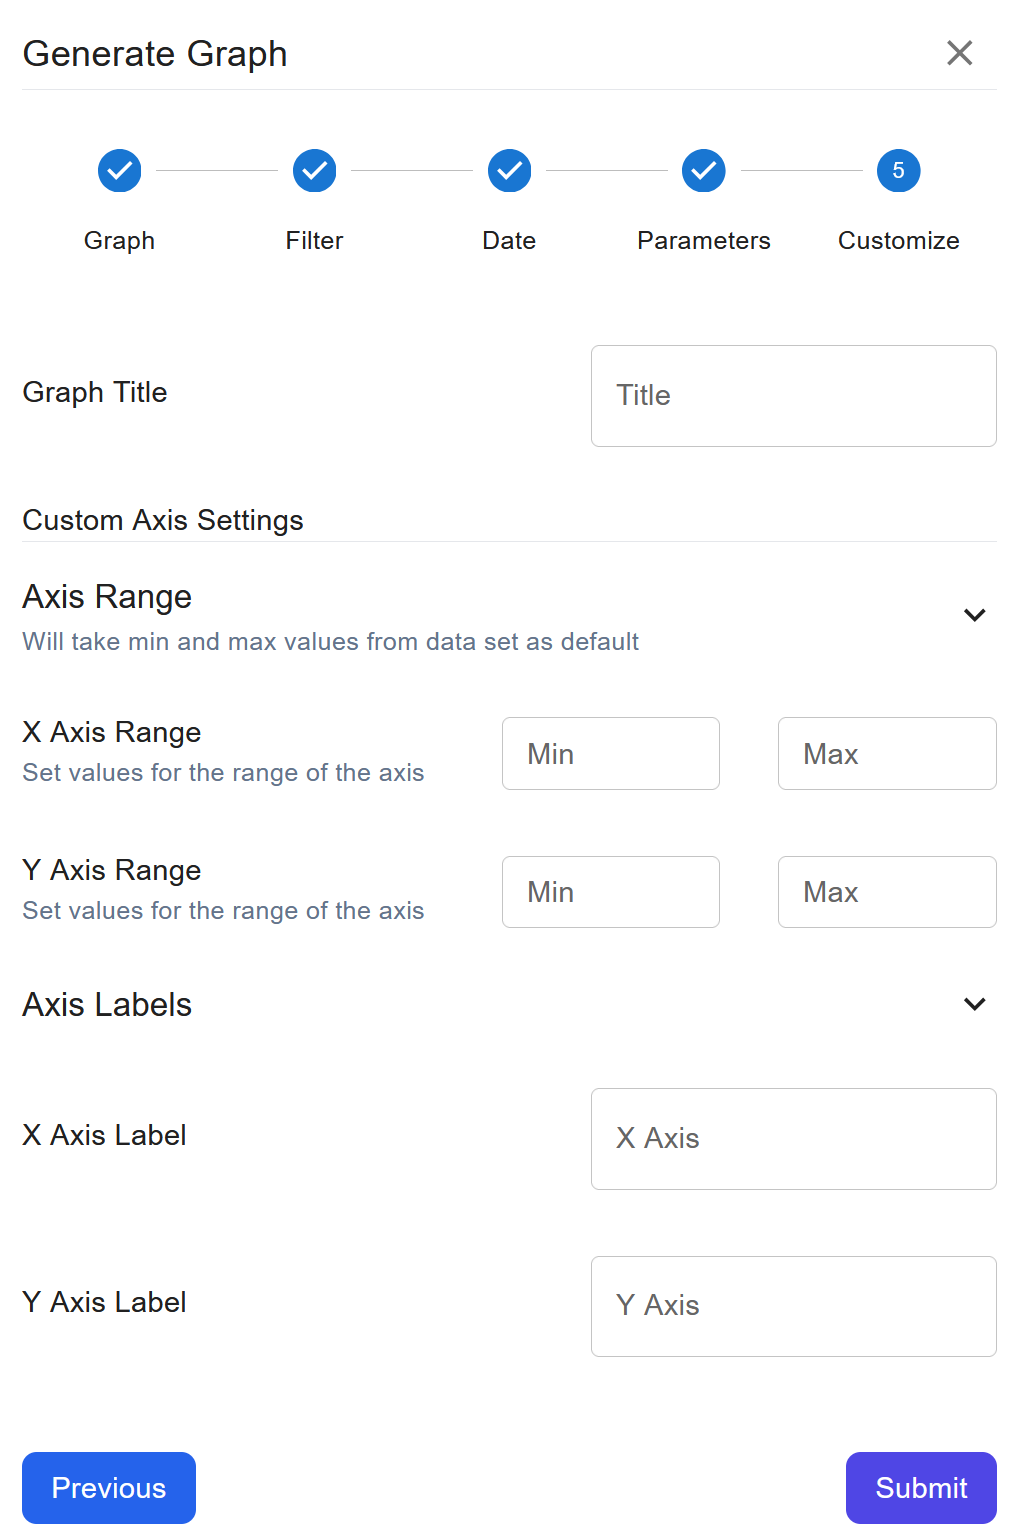
\includegraphics[scale=0.6]{Images/graph-custom.png}
        \caption{Sample Input of the Filter Step}
        \label{fig:example}
    \end{figure}
\end{enumerate}

\section{Troubleshooting}

This section lists common issues, error messages, and their solutions, along
with advanced diagnostic procedures.

\subsection{Common Graphing Issues}

\begin{table}[H]
    \centering
    \begin{tabularx}{\textwidth}{lXl}
        \toprule
        \textbf{Issue} & \textbf{Solution} \\
        \midrule
        Dropdown options not appearing & There may be no value for the
        selected combination of attributes or filters. Check to verify inputted
        options \newline \\
        Frozen form & There may be a large number of options to select from.
        Please give the page a few minutes to finishing loading up and
        displaying all the data \newline \\
        Rendering failed & Validate data selection \\
        \bottomrule
    \end{tabularx}
\end{table}
\end{document}